
\subsection{Properties of \acs{BSCO}}

The unit cell of the \highTc, doped cuprate \acf{BSCO} is illustrated in figure~\ref{Fig:Intro:BSCOUnitCell}. It is made up of layers as follows from the top; a BiO layer, then a SrO layer, then a CuO lattice common to all cuprates, then 2 BiO layers, a SrO layer, CuO, SrO, BiO. Variants of \acs{BSCO} include \ac{BSCO2212} and \ac{BSCO2213} which feature one and two extra CuO layers respectively. Most closely related in terms of structure is \acs{TL2201} which features Tl and Ba in place of Bi and Sr respectively.
\begin{figure}[htbp]
    \begin{center}
        \includegraphics[scale=1.1]{Chapter-Introduction/Figures/BSCOUnitCell/BSCOUnitCell}
        \caption{Unit cell of \acs{BSCO} demonstrating the layers. \ac{TL2201} is similar but with La for Bi and Ba for Sr. Note that Pb doping occurs away from the CuO planes.}
        \label{Fig:Intro:BSCOUnitCell}
    \end{center}
\end{figure}
Undoped \ac{BSCO} has an excess of holes and lies slightly to the undoped side of the phase diagram. By substituting in La for Sr, the amount of holes is reduced allowing access to a range of slightly overdoped to underdoped. However, since the substitution takes place adjacent to the CuO planes where all the interesting electronic behaviour happens, La doping introduces a lot of disorder into the system. Pb is also substituted for Bi which increases the number of holes allowing the more overdoped region to be accessed. Since Pb substitutes into the BiO layer which is far from the CuO plane, less disorder is introduced. Sometimes Pb is introduced alongside La even when a more underdoped state is desired to avoid forming structures in the BiO planes which affect \ac{ARPES} measurements~\cite{Kondo2007}. Furthermore, annealing in oxygen decreases the number of carriers depending on how much additional oxygen is absorbed allowing for even more fine grained tuning of the doping. By adjusting these parameters a very wide range of doping values can be accessed in \ac{BSCO} which makes it appealing for study.

The precise determination of doping from a chemical standpoint is tricky. For \ac{LSCO} --- assuming pure ionic donation --- substituting more Sr for La simply adds one more hole per extra Sr atom per unit cell. However for \ac{Y123} and \ac{Y124} for example, there exist CuO chains (oxygen deficient CuO layers) which absorb some of the doped charge, other cuprates the heavy metal atom has a mixed valency meaning that the substitution relation is not so straightforward. Various techniques described in the methods section have been described to determine the doping level but as a rule some a priori knowledge of composition is required.
\begin{figure}[htbp]
    \begin{center}
        \includegraphics[scale=0.9]{Chapter-Introduction/Figures/VanHoveBSCOLSCO/VanHoveBSCOLSCO}
        \caption{Band dispersions at the Fermi energy for various dopings. Left panel shows \ac{BSCO}, right panel shows \ac{LSCO}. Note the saddle points at $(\pi, 0)$ which cause the van-Hove singularity at $p\approx 0.18$ for \ac{LSCO} and at $p \geq 0.2$ for \ac{BSCO}. Adapted from ref~\cite{Hashimoto2008}.}
        \label{Fig:Intro:VanHoveBSCOLSCO}
    \end{center}
\end{figure}
There is a crossover in overdoped cuprates between a large hole-like Fermi surface to an electron-like Fermi surface that leads to a saddle point in the \ac{DOS} and consequently a van Hove singularity (see figure~\ref{Fig:Intro:VanHoveBSCOLSCO}, adapted from ref.~\cite{Hashimoto2008}). This occurs in \ac{LSCO} at around $p=0.18$ which is approximately critical doping and may lead one to believe that the critical behaviour is related to the proximity of the van Hove singularity. However the same crossover does not happen at the same doping in \ac{BSCO}, rather it appear to occur at $p \geq 0.2$, relatively far from the critical value of $p \approx 0.16$. For this reason \ac{BSCO} is an attractive material to study to determine more about the relationship (or lack thereof) between the critical behaviour and the van Hove singularity.

Finally \ac{BSCO} has a relatively low maximum \Tc, being around \unit{36}{\kelvin} at best. Because \Tc is so low, this makes \ac{BSCO} ideal for normal state study since less field will be required to suppress \Tc at lower temperatures.
